\documentclass[11pt,a4paper]{article}
\usepackage[german]{babel}
\usepackage[utf8]{inputenc}
\usepackage[T1]{fontenc}
\usepackage{amsmath,amssymb,amsfonts}
\usepackage{graphicx}

% Blackboard bold symbols (formerly from mathsym.sty at IAKS Karlsruhe)
\newcommand{\R}{{\mathbb{R}}}
\newcommand{\C}{{\mathbb{C}}}

\newcommand{\betrag}[1]{|#1|}
\newcommand{\fourier}[1]{\mathcal{F}\left( #1\right)}
\newcommand{\norm}[1]{\parallel #1 \parallel_{W_{Signal}}}
\newcommand{\snr}[2]{\mbox{SNR}_I ( #1, #2 )}
\newcommand{\skalar}[2]{\left< #1, #2 \right>_{W_{Signal}}}

\begin{document}

\pagestyle{empty}
\advance\rightmargin22mm
{\Large
\begin{center}
\vspace*{1cm}

{\huge\bf Entwurf diffraktiver Strahlformer mit der Methode der finiten Elemente} \\[1cm]
\begin{figure}[htb]
   \centerline{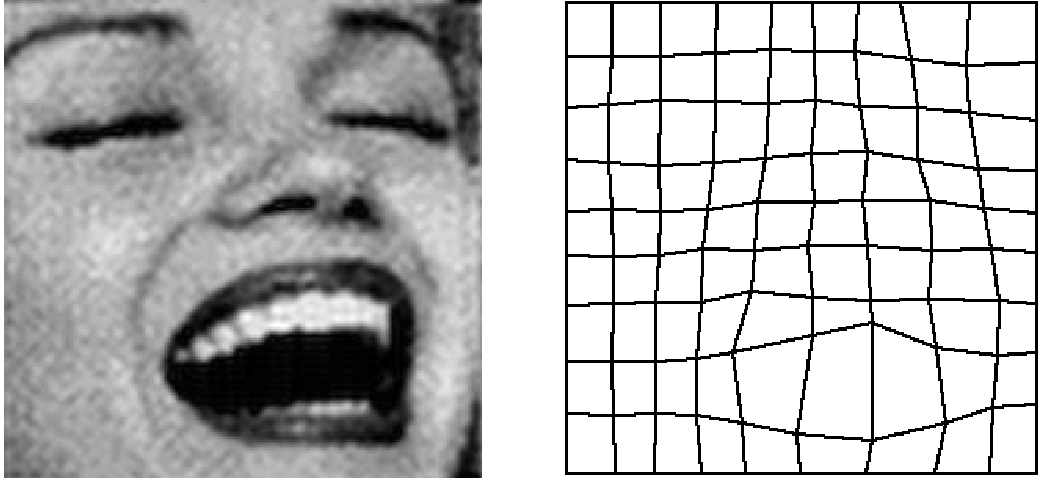
\includegraphics[width=6cm]{titelbild}}
\end{figure}
{\em Eine Studienarbeit von}\\[1cm]
{\LARGE\bf Pawel Wocjan}\\[1cm]
{\em am}\\[1cm]
{\LARGE Institut f"ur Algorithmen und Kognitive Systeme}\\
{\LARGE Fakult"at f"ur Informatik, Universit"at Karlsruhe (TH)}\\[1cm]
{\em unter Betreuung von}\\[1cm]
{\LARGE Prof.~Dr.~Th.~Beth}\\
{\LARGE Dipl.--Inform.~M.~Schmid}\\
\vfill

Sommersemester 1997\\
\vfill\vfill
\end{center}
}

\newpage
\thispagestyle{empty}
\mbox{}
\newpage
\tableofcontents
\newpage
\mbox{}
\newpage
\pagestyle{plain}

\section{Einf"uhrung} 
  Eines der grundlegenden Probleme der diffraktiven Optik ist es, ein
  diffraktives Element (DE) mit der Transmissionsfunktion $T_{DE}$ zu
  finden, die zu einem gegebenen Eingabesignal $f_1$ ein zuvor definiertes 
  Ausgabesignal $f_2$ erzeugt. Die Transmissionsfunktion $T_{DE}$ ist eine 
  komplexe Funktion der reellen Ebene, d.h.
  $$ T_{DE} : \left\{
                 \begin{array}{rcl}
                  \R^2  & \longrightarrow & \C \\
                  (x,y) & \longmapsto     & A(x,y) \exp (i\phi (x,y)).
                 \end{array}
               \right.
  $$ 
  Die Amplitude $A(x,y)$ nimmt Werte aus dem Bereich $[0,1]$ an, wobei 0 v"ollige Absorption
  und 1 v"ollige Transparenz bedeutet. Die Phasenverz"ogerung $\phi(x,y)$ stammt
  aus dem Bereich $[0,2\pi)$. In vielen praktischen F"allen ist nur
  die Intensit"at des Ausgabesignals $\betrag{f_2}$ wichtig, die
  Phase kann beliebig sein.  Wenn man von dem optischen Aufbau in 
  Abbildung~\ref{aufbau} ausgeht, wird 
  also eine Transmissionsfunktion $T_{DE}$ gesucht, die 
  $$ \fourier{T_{DE} f_1} = f_2 $$
  erf"ullt. Die Wellenausbreitung wird durch die Fouriertransformation $\mathcal{F}$
  beschrieben (siehe \cite{diplom}).
    
  \begin{figure}[htb]
    \centerline{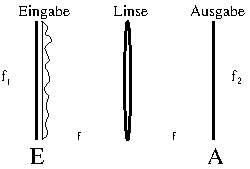
\includegraphics{aufbau}}
    \caption{Die Eingabe- und Ausgabeebene befinden sich im Abstand $f$ von der Linse.}\label{aufbau}
  \end{figure}

  Leider kann nicht jede Transmissionsfunktion $T_{DE}$ technisch realisiert werden. 
  Die vorhandenen Mittel schr"anken die Klasse der herstellbaren diffraktiven 
  Elemente deutlich ein. Diffraktive Elemente, die sowohl die Amplitude als auch 
  die Phase modulieren, lassen sich noch nicht zufriedenstellend herstellen. Deshalb 
  mu"s man sich in der Regel auf diffraktive Amplitudenelemente oder diffraktive 
  Phasenelemente beschr"anken. Die Amplitudenelemente haben den gro"sen Nachteil 
  der Energieabsorption. Die Energie des Signals $f_1$ kann nicht vollst"andig
  f"ur das Signal $f_2$ ausgenutzt werden. Au"serdem wird das diffraktive 
  Amplitudenelement erw"armt, was bei gro"sen Energiemengen, 
  die bei manchen Anwendungen zur Materialverarbeitung auftreten, 
  sogar zur Zerst"orung f"uhren kann.	

  Im folgenden werden nur Phasenelemente behandelt, die im Idealfall keine Energie, 
  in der Realit"at jedoch eine geringe Menge, absorbieren. Ein diffraktives
  Phasenelement (DPE) wird durch eine Transmissionsfunktion $T_{DPE}$
  $$ T_{DPE} : \left\{
                 \begin{array}{rcl}
                  \R^2  & \longrightarrow & \C \\
                  (x,y) & \longmapsto     & \exp (i\phi (x,y))
                 \end{array}
               \right.
  $$ 
  beschrieben, wobei die Phasenfunktion $\phi(x,y)$ die Phasenverteilung angibt.

\section{Die Methode der station"aren Phase} 
  Wir wollen die Phasenfunktion $\phi(x,y)$ eines Phasenelements bestimmen, das einen
  Punkt $T(x,y)$ der Ausgabeebene $A$ ausleuchtet, wenn im Punkt $(x,y)$ der 
  Eingabeebene $E$ beleuchtet wird (siehe Abbildung \ref{transform}).
  \begin{figure}[htb]
    \centerline{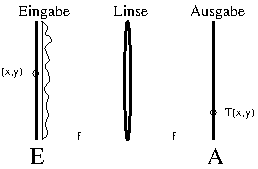
\includegraphics{transf}}
    \caption{Realisierung einer geometrischen Transformation $T$ mit einem DPE}\label{transform}
  \end{figure}
  Es soll also ein Phasenelement berechnet
  werden, das eine gegebene geometrische Transformation $T$ von der Eingabe- in die
  Ausgabeebene realisiert. Nach der Methode der station"aren Phase (siehe \cite{diplom} und
  \cite{analytisch}) mu"s die Phasenverteilung 
  $\phi(x,y)$ im kontinuierlichen Fall so gew"ahlt werden, da"s
  $$ \nabla\phi(x,y) = \frac{2\pi}{\lambda f} T(x,y) $$
  gilt, um die geometrische Transformation $T$ zu realisieren. Die Wellenl"ange ist $\lambda$.

\section{Analytische L"osungen}
  Betrachten wir das Problem, eine beliebige Wellenfront $f_1$ in eine Wellenfront $f_2$,
  bei der nur die Intensit"at vorgegeben ist, mit einem diffraktiven Phasenelement
  zu transformieren. Da die Phase der Wellenfront $f_1$ im Phasenelement 
  codiert werden kann, nehmen wir ab jetzt oBdA an, da"s die Phase von $f_1$ 
  konstant ist. 

  Bei den analytischen Algorithmen (siehe \cite{analytisch}) wird im ersten Schritt 
  eine geometrische Transformation $T$ berechnet, die die Intensit"at $\betrag{f_1}$ in die Intensit"at
  $\betrag{f_2}$ umverteilt. Die Abbildung~\ref{umverteilung} soll dem intuitiven
  Verst"andnis der Idee der Energieumverteilung dienen. 

  \begin{figure}[htb]
    \centerline{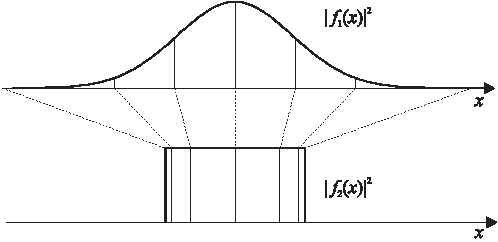
\includegraphics{distort}}
    \caption{Energieumverteilung durch eine geometrische Transformation~$T$.}\label{umverteilung}
  \end{figure}
    
  Allerdings kann diese geometrische Transformation $T$ nicht f"ur
  beliebige Wellenfronten berechnet werden. Es k"onnen nur Transformationen eines 
  separablen Eingabesignals in ein separables Ausgabesignal oder eines 
  isotropen Eingabesignals in ein isotropes Ausgabesignal berechnet werden, da sich
  dann die Transformation $T$ auf einen einfachen eindimensionalen Fall 
  zur"uckf"uhren l"a"st.

  Im zweiten Schritt wird mit der Methode der station"aren Phase die 
  Phasenfunktion $\phi(x,y)$ des Phasenelements berechnet, das die
  geometrische Transformation $T$ realisiert.

  Die Idee des Separabilisierungsoperators SepOp erlaubt es, eine geeignete geometrische 
  Transformation $T$ zu berechnen, auch wenn die Wellenfronten nicht in den
  obigen Klassen liegen. Dazu werden beliebige Signale auf m"oglichst "ahnliche
  separable Signale abgebildet. 
  $$ \mbox{SepOp : } f(x,y) \mapsto \int_{\xi_1=-\infty}^\infty f(\xi_1,y) d\xi_1 
                                    \int_{\xi_2=-\infty}^\infty f(x,\xi_2) d\xi_2 $$
  Ein Beispiel ist in Abbildung~\ref{sepop} dargestellt.
  Wenn wir das Signal auf ein separables Signal abgebildet haben, 
  k"onnen wir die analytische Methode anwenden. 
  \begin{figure}[htb]
    \centerline{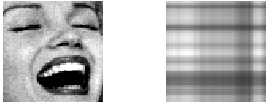
\includegraphics[width=8cm]{MaSepOp}}
    \caption{Abbildung eines nichtseparablen Signals auf ein "ahnliches separables Signal.}\label{sepop}
  \end{figure}

  Das so erhaltene Phasenelement erzeugt ein bereits "ahnliches Signal zu $f_2$ und stellt somit
  einen guten Startwert f"ur den iterativen Fouriertrans\-formationsalgorithmus (IFTA) (siehe
  \cite{ifta1}, \cite{ifta2} und \cite{ifta3}), der es noch weiter optimiert.

  Die Methode der finiten Elemente soll eingesetzt werden, falls die
  geometrische Transformation $T$ nicht analytisch berechnet werden kann.
  Mit ihr sollen g"unstigere Startwerte f"ur den IFTA als mit dem 
  Separabilisierungsoperator erreicht werden.

\section{Die Methode der finiten Elemente}
  Wir unterteilen die Ebene $E$ und die Ebene
  $A$ in finite Fl"achenelemente. Zu jedem Fl"achenelement der Eingabeebene $E$ gibt es
  ein korrespondierendes Fl"achenelement der Ausgabeebene $A$. Wenn es uns gelingt, die Fl"achenelemente
  derart anzuordnen, da"s jeweils korrespondierende Fl"achenelemente die gleiche Energie enthalten und
  dann eine geometrische Transformation berechnen, die die Energie der Fl"achenelementen der
  Ebene $E$ in jeweils korrespondierenden Fl"achenelemente der Ebene $A$ umlenkt, k"onnen wir das
  gew"unschte Phasenelement realisieren. 

  Bei der Anwendung der finiten Elemente f"ur den Entwurf von 
  diffraktiven Elementen m"ussen wir zun"achst eine f"ur das vorliegende Problem 
  geeignete Netztopologie ausw"ahlen. Ein Netz wird durch eine diskrete Anzahl von
  Netzknoten, die eindeutig durch ein Paar $(i,j)$ adressiert werden, gebildet. Das Paar
  $(i,j)$ stammt aus einem von der Topologie abh"angigen Defini\-tionsbereich. 

  Wir legen "uber die Eingabeebene $E$ und die Ausgabeebene $A$ zwei topologisch "aquivalente 
  Netze, indem wir f"ur alle $(i,j)$-Paare die Koordinaten $(x_{ij},y_{ij})$ der 
  Knoten $in(i,j)$ des Netzes in der Eingabeebene $E$ und die Koordinaten 
  $(\phi_x^{ij},\phi_y^{ij})$ der Knoten $out(i,j)$ des Netzes in der Ausgabebene
  $A$ festlegen.

  Die Netzknoten $in(i,j)$ und $out(i,j)$ bilden finite Fl"achenelemente, deren Form 
  von der jeweils gew"ahlten Netztopologie abh"angt. Jedes finite Fl"achenelement
  unterteilt die Ebene $E$ bzw. $A$ und enth"alt eine bestimmte Energie. Wenn es uns gelingt
  die beiden Netze so zu optimieren, da"s korrespondierende Fl"achenelemente in der Ebene $E$ und $A$ 
  die gleiche Energie einschlie"sen, k"onnen wir mit der Approximation der station"aren Phase 
  die Phasenfunktion $\phi(x,y)$ eines Phasenelements berechnen, das die gew"unschte Transformation
  realisiert. 

  \subsection{Netze mit Rechteckstopologie}
    Zun"achst werden zwei Spezialf"alle aus \cite{finite} vorgestellt. Die darin
    verwendeten Methoden werden dahingehend erweitert, da"s wir Netze f"ur Wellenfronten mit
    beliebigen Intensit"atsverteilungen generieren k"onnen.

    Betrachten wir das Problem, einen Kreis mit konstanter Intensit"at in ein Quadrat mit 
    konstanter Intensit"at zu transformieren. Da die Intensit"at innerhalb der beiden Figuren
    konstant ist, schlie"sen gleich gro"se Fl"achenelemente gleich viel Energie ein. 

    Ein Netz mit Rechteckstopologie ist in Abbildung~\ref{rechttop} gezeigt. Die Werte f"ur $i,j$ stammen
    aus dem Bereich $0,\ldots,s-1$, wobei $s$ die Gesamtanzahl der Netzknoten in einer
    Richtung angibt.
    \begin{figure}[htb]
      \centerline{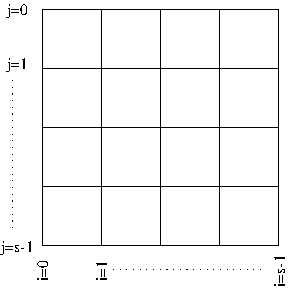
\includegraphics{rechttop}}
      \caption{Rechteckstopologie}\label{rechttop}
    \end{figure}
    Wir legen "uber das Quadrat in der Ausgabeebene $A$ ein Netz, d.h. wir definieren eine 
    Abbildung, die jedem $(i,j)$-Paar die Koordinaten $(\phi_x^{ij},\phi_y^{ij})$ des 
    Knotens~$out(i,j)$ zuordnet. Die Werte der Koordinaten $(\phi_x^{ij},\phi_y^{ij})$ stammen aus dem
    Bereich $\left[ -0.25, 0.25\right]$. Die Koordinaten $(\phi_x^{ij},\phi_y^{ij})$ werden so 
    gew"ahlt, da"s das Quadrat in gleich gro"se quadratische Fl"achenelemente unterteilt wird und sein  
    Schwerpunkt im Ursprung liegt.

    Wir m"ussen nun ein Netz "uber den Kreis in der Eingabeebene $E$ so legen, da"s 
    alle finiten Fl"achenelemente gleich gro"s sind. Diese Aufgabe wird mit einem
    Netzgenerierungsalgorithmus gel"ost, der aus den folgenden drei Schritten
    besteht:
    \begin{enumerate}
      \item Bestimmung der Abbildung f"ur die Randknoten.
      \item Generierung der inneren Knoten mit einer Interpolationstechnik.
      \item Iterative Bewegung der Knoten, um Randbedingungen zu erf"ullen.
    \end{enumerate}
    Der erste Schritt ist einfach zu realisieren, indem wir die Randknoten
    auf einem Ursprungskreis mit Radius $r=0.25$ gleichm"a"sig anordnen. Der zweite Schritt 
	wird mit der Vier-Punkt-Interpolationstechnik aus \cite{atkin} realisiert. Ein innerer Knotenpunkt 
    $P_0 = (x_0, y_0)$ wird durch seine vier zugeh"origen Randknoten 
    $P_l=(x_l, y_l), l=1,\ldots,4$ (siehe Abbildung~\ref{vier}), interpoliert
    \begin{equation} P_0 :=\sum_{l=1}^4 g_l P_l. \label{vierinterpol} \end{equation}
    \begin{figure}[htb]
      \centerline{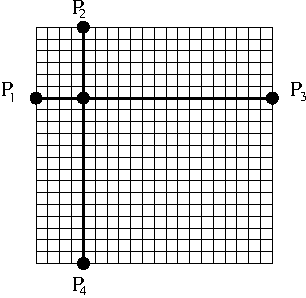
\includegraphics{vier}}
      \caption{Die vier zugeh"origen Randknoten.}\label{vier}
    \end{figure}
    Die Gewichte $g_l$ werden durch folgende Formeln 
    \begin{eqnarray*}
      g_1 & = & \frac{d_2  d_3  d_4}{(d_1 + d_2)  (d_1  d_2 + d_3  d_4)} \\
      g_2 & = & \frac{d_1  d_3  d_4}{(d_1 + d_2)  (d_1  d_2 + d_3  d_4)} \\
      g_3 & = & \frac{d_1  d_2  d_4}{(d_3 + d_4)  (d_3  d_4 + d_1  d_2)} \\
      g_4 & = & \frac{d_1  d_2  d_3}{(d_3 + d_4)  (d_3  d_4 + d_1  d_2)}
    \end{eqnarray*}
    bestimmt. Die  $d_k := [(i_0-i_k)^2+(j_0-j_k)^2]^{1/2}$ sind die euklidischen
    Abst"ande im $(i,j)$-Bereich. Die Interpolationsformel~\ref{vierinterpol} ist linear in den Koordinaten 
	der Randpunkte $P_1,\ldots,P_4$. Das Netz, das nach den ersten beiden Schritten
    des Generierungsalgorithmus f"ur $s=20$ entsteht, ist in Abbildung~\ref{mesh1} dargestellt. 
    \begin{figure}[htb]
      \centerline{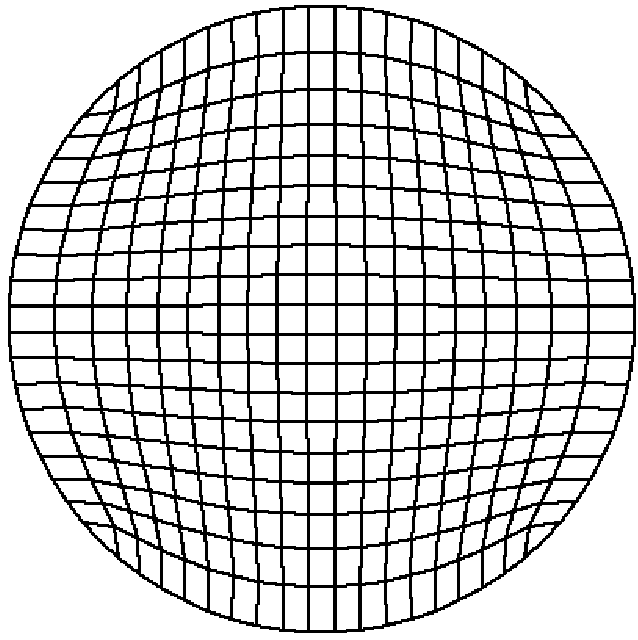
\includegraphics[width=4cm]{mesh1}}
      \caption{Das mit der Vier-Punkt-Interpolationstechnik berechnete Netz.}\label{mesh1}
    \end{figure}
    Viele Netzgenerierungsalgorithmen gl"atten die Verteilung der inneren
    Knoten mit Hilfe des diskreten Laplaceoperators. Das Netz nach der Laplace-Gl"attung ist in 
    Abbildung~\ref{mesh2} gezeigt. 
    \begin{figure}[htb]
      \centerline{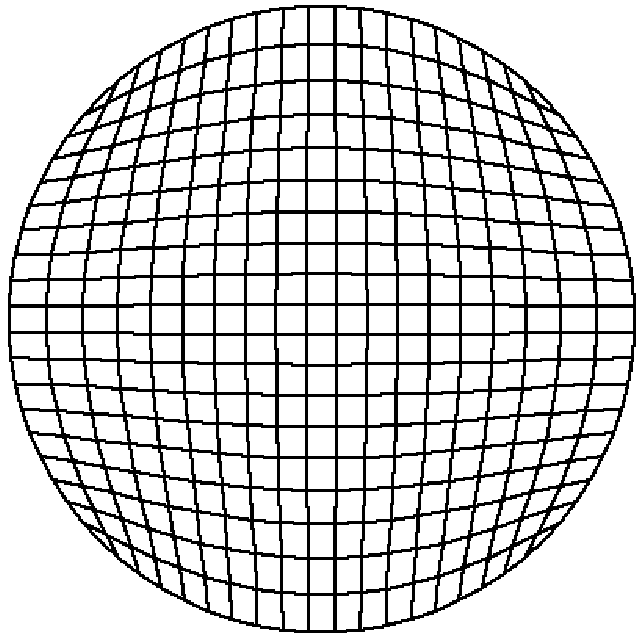
\includegraphics[width=4cm]{mesh2}}
      \caption{Das mit dem Laplaceoperator gegl"attete Netz.}\label{mesh2}
    \end{figure}
    Ein innerer Knoten $P_0$ ist von vier 
    Nachbarn $P_k = (x_k, y_k), k=1\ldots,4$ (siehe Abbildung~\ref{schwer}) umgeben. 
    Der Schwerpunkt $C=(x_c, y_c)$ dieser Knoten befindet sich in
    \begin{equation} C:=\frac{1}{4}(P_1 + P_2 + P_3 + P_4). \end{equation}
    Die Differenz von $P_0$ und $C$ ist $D:=C-P_0$. Sie ist die diskrete
    Vier-Punkt-Approximation des Laplaceoperators im zweidimensionalen Fall.
    Der innere Knoten $P_0$ wird in Richtung von $C$ bewegt, d.h.
    \begin{equation} P_0' := P_0 + \alpha D, \label{verschiebung} \end{equation}
    so da"s die neue Differenz $D' := C - P_0'$ kleiner wird. Die Konstante $\alpha$ 
    kontrolliert die Schrittweite im Algorithmus. 
    \begin{figure}[htb]
      \centerline{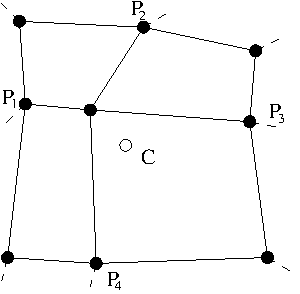
\includegraphics{schwer}}
      \caption{Der innere Knoten $P_0$ ist von den vier Nachbarpunkten $P_1,\ldots, P_4$ umgeben}
      \label{schwer}
    \end{figure}
    Wie kann dieses Verfahren verwendet werden, um ein Netz mit gleich gro"sen
    Fl"achenelementen zu erhalten? Betrachten wir einen inneren Punkt $P_0$ und seine acht 
    Nachbarpunkte $P_1,\ldots,P_8$ (siehe Abbildung~\ref{acht}).
    \begin{figure}[htb]
      \centerline{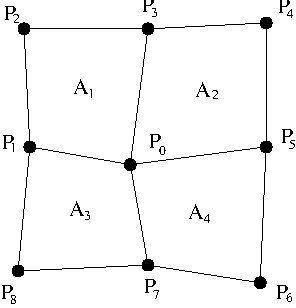
\includegraphics{acht}}
      \caption{Acht Nachbarknoten eines inneren Knotens $P_0$}\label{acht}
    \end{figure}
    Um gleich gro"se Fl"achenelemente zu erhalten, fordern wir, da"s die ideale Position $C$ f"ur den 
    inneren Punkt $P_0$ so gew"ahlt wird, da"s die Fl"achen $A_1,\ldots,A_4$ folgende Gleichungen 
    \begin{eqnarray}
      A_1 + A_2 & = & A_3 + A_4 \\
      A_1 + A_3 & = & A_2 + A_4
    \end{eqnarray}
    erf"ullen. Diese Gleichungen sind zu den Bedingung $A_1 = A_4$ und
    $A_2 = A_3$ "aquivalent. Wenn sie f"ur alle inneren Knoten gleichzeitig
    erf"ullt sind, erhalten wir ein "`Schachbrett"', bei dem alle schwarzen und alle wei"sen Rechtecke gleich
    gro"s sind. Alle Rechtecke sind dann fast gleich gro"s. Wenn wir die beiden Gleichungen in 
    den Koordinaten der 
    acht Nachbarknoten $P_1,\ldots,P_8$ und der idealen Position $C(x_c, y_c)$ ausdr"ucken, bekommen wir zwei 
    lineare Gleichungen. Die L"osung f"ur die Koordinaten $x_c$ und $y_c$ sind dann
    \begin{eqnarray}
       x_c & = & \frac{b f - d e}{b c - a d} \\
       y_c & = & \frac{a f - c e}{b c - a d},
    \end{eqnarray}
    wobei
    \begin{eqnarray*}
       a & = & y_2 - y_8 - y_6 + y_4 \\
       b & = & x_2 - x_8 - x_6 + x_4 \\
       c & = & y_8 - y_6 - y_4 + y_2 \\
       d & = & x_8 - x_6 - x_4 + x_2 \\
       e & = & x_1 \cdot (y_2 - y_8) + x_5 \cdot (y_4 - y_6) + y_1 \cdot (x_8 - x_2) + y_5 \cdot (x_6 - x_4) \\
       f & = & x_3 \cdot (y_2 - y_4) + x_7 \cdot (y_8 - y_6) + y_3 \cdot (x_4 - x_2) + y_7 \cdot (x_6 - x_8).
    \end{eqnarray*}
    gesetzt sind. Wir definieren wieder $D := C - P_0$ als 
    die Abweichung von $P_0$ von der idealen Position $C$. Die neue Position $P_0'$
    wird wie in Gleichung~\ref{verschiebung} definiert. Dieser Schritt wird so lange f"ur alle inneren
    Knoten wiederholt, bis sie sich nicht mehr bewegen. Das so entstandene Netz ist in 
    Abbildung~\ref{mesh3} gezeigt. 
    \begin{figure}[htb]
      \centerline{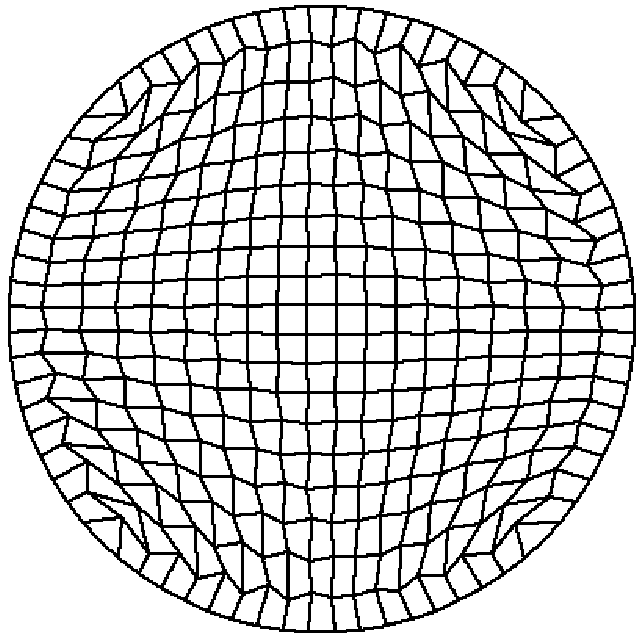
\includegraphics[width=4cm]{mesh3}}
      \caption{Das bei der Abbildung eines Quadrats auf einen Kreis entstandene Netz. Das Netz wurde dabei so optimiert, da"s alle Fl"achenelemente gleich gro"s sind.}\label{mesh3}
    \end{figure}
    Bei diesem Algorithmus wurden die Randknoten nicht bewegt. Wir erhalten ein
    besseres Ergebnis, wenn auch die Randknoten bewegt werden. Betrachten wir einen
    Randknoten, der kein Eckpunkt ist. Dieser Knoten hat f"unf Nachbarn (siehe Abbildung~\ref{rechtran}). 
    \begin{figure}[htb]
      \centerline{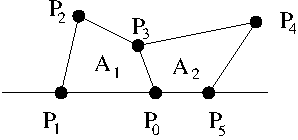
\includegraphics{rechtran}}
      \caption{F"unf Nachbarpunkte eines Randknotens.}\label{rechtran}
    \end{figure}
    Die Bedingung $A_1 = A_2$ ergibt eine lineare Gleichung f"ur die Koordinaten 
    $x_c$ und $y_c$ der idealen Position $C$ 
    \begin{equation} a x_c + b y_c = e, \end{equation}
    wobei
    \begin{eqnarray*}
      a & = &  y_1 - 2  y_3 + y_5  \\
      b & = & -x_1 + 2  x_3 - x_5 \\
      e & = &  x_3  y_4 - y_3  x_4 + x_4  y_5 - y_4  x_5 - ( x_1  y_2 - y_1  x_2 + x_2  y_3 - y_2 x_3 ).
    \end{eqnarray*}
    Wir wissen nun, auf welcher Geraden die ideale Position $C$ liegt. Die zweite Bedingung,
    die die ideale Position $C$ festlegt, ergibt sich aus der Tatsache, da"s der Knoten auf dem 
    Kreis liegen mu"s. Es gibt zwei Schnittpunkte der Geraden mit dem Kreis. Es
    wird der Schnittpunkt genommen, der die kleinere Entfernung zu den Knoten $P_1$ und $P_5$ 
    hat. Hier kann nicht die Gleichung~\ref{verschiebung} benutzt werden, um den Knoten
    $P_0$ in Richtung $C$ zu bewegen, da sonst die neue Position $P_0'$ nicht auf dem
    Kreis liegen w"urde. Es wird daher die Differenz des Winkels zwischen $P_0$ und $C$
    betrachtet. Das Netz, bei dem auch die Randknoten bewegt wurden, ist in Abbildung~\ref{mesh4} 
    dargestellt. Das Ergebnis ist geringf"ugig besser.
    \begin{figure}[htb]
      \centerline{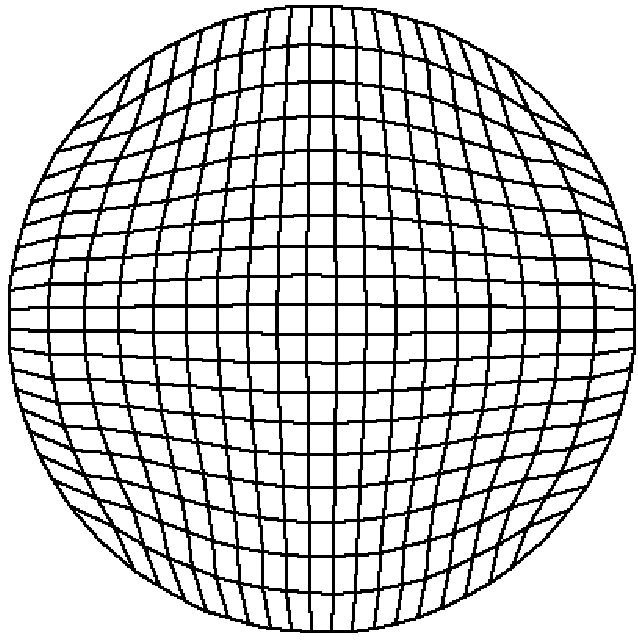
\includegraphics[width=4cm]{mesh4}}
      \caption{Das bei der Abbildung eines Quadrats auf einen Kreis entstandene Netz. Das Netz wurde dabei so optimiert, da"s alle Fl"achenelemente gleich gro"s sind.}\label{mesh4}
    \end{figure}
%%
%%  Netze mit Dreieckstopologie   
%%
  \subsection{Netze mit Dreieckstopologie}
    Betrachten wir das Problem, einen Kreis mit konstanter Intensit"at in ein Dreieck mit konstanter Intensit"at
    zu transformieren. F"ur die L"osung dieses Problems ist die Rechteckstopologie nicht mehr geeignet, 
    da es sehr umst"andlich w"are, das Dreieck mit Rechtecken auszuf"ullen. Es ist viel einfacher dreieckige 
    Fl"achenelemente zu benutzen.

    Es werden nur die notwendigen "Anderungen im Konzept beschrieben, 
    um Netze mit einer Dreieckstopologie zu optimieren. Ein Netz mit Dreiecks\-topologie ist in
    Abbildung~\ref{dreitop} dargestellt. Der Definitionsbereich der $(i,j)$-Paare  mu"s
    ge"andert werden. Die Netzknoten werden hier durch
    $(i,j)$-Paare bezeichnet, wobei $j$ die Werte $j=0,\ldots,s-1$ und $i$ die
    Werte $i=0,\ldots,j$ annehmen. Die Gesamtzahl der Zeilen wird mit $s$ bezeichnet.
    \begin{figure}[htb]
      \centerline{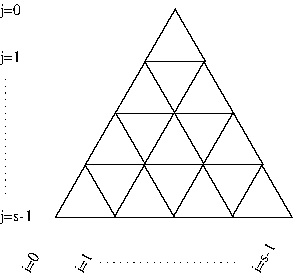
\includegraphics{dreitop}}
      \caption{Dreieckstopologie}\label{dreitop}
    \end{figure}
    Es wird ein Sechs-Punkt-Algorithmus aus \cite{finite} verwendet, bei dem ein 
    innerer Knoten $P_0$ durch seine sechs zugeh"origen Randknoten $P_1,\ldots,P_6$
    (siehe Abbildung~\ref{sechs})
   \begin{equation} P_0 := \sum_{l=1}^6 g_l P_l \label{sechsinterpol} \end{equation}
   interpoliert wird.
   \begin{figure}[htb]
      \centerline{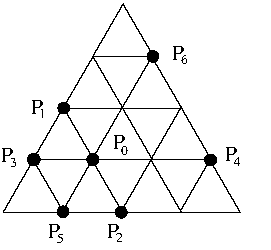
\includegraphics{sechs}}
      \caption{Die sechs zugeh"origen Randknoten zu dem inneren Randknoten $P_0$}\label{sechs}
    \end{figure}
    Die Gewichte werden mit folgenden Formeln
    \begin{eqnarray*}
      g_1 = \frac{d_2  d_3  d_4  d_5  d_6}{(d_1 + d_2)  (d_1  d_2 + d_3  d_4)  (d_1  d_2 + d_5  d_6)} \\
      g_2 = \frac{d_1  d_3  d_4  d_5  d_6}{(d_1 + d_2)  (d_1  d_2 + d_3  d_4)  (d_1  d_2 + d_5  d_6)} \\
      g_3 = \frac{d_1  d_2  d_4  d_5  d_6}{(d_3 + d_4)  (d_3  d_4 + d_1  d_2)  (d_3  d_4 + d_5  d_6)} \\
      g_4 = \frac{d_1  d_2  d_3  d_5  d_6}{(d_3 + d_4)  (d_3  d_4 + d_1  d_2)  (d_3  d_4 + d_5  d_6)} \\
      g_5 = \frac{d_1  d_2  d_3  d_4  d_6}{(d_5 + d_6)  (d_5  d_6 + d_1  d_2)  (d_5  d_6 + d_3  d_4)} \\
      g_6 = \frac{d_1  d_2  d_3  d_4  d_5}{(d_5 + d_6)  (d_5  d_6 + d_1  d_2)  (d_5  d_6 + d_3  d_4)} 
    \end{eqnarray*}
    berechnet. Die Interpolationsformel~\ref{sechsinterpol} ist linear in den Koordinaten der
    Knoten $P_1,\ldots,P_6$. Die Gewichte $d_k$ h"angen von der
    Entfernung des Knoten von den zugeh"origen Randknoten $P_1,\ldots,P_6$ ab.
    Das damit berechnete Netz ist in Abbildung~\ref{tmesh1} dargestellt.
    \begin{figure}[htb]
      \centerline{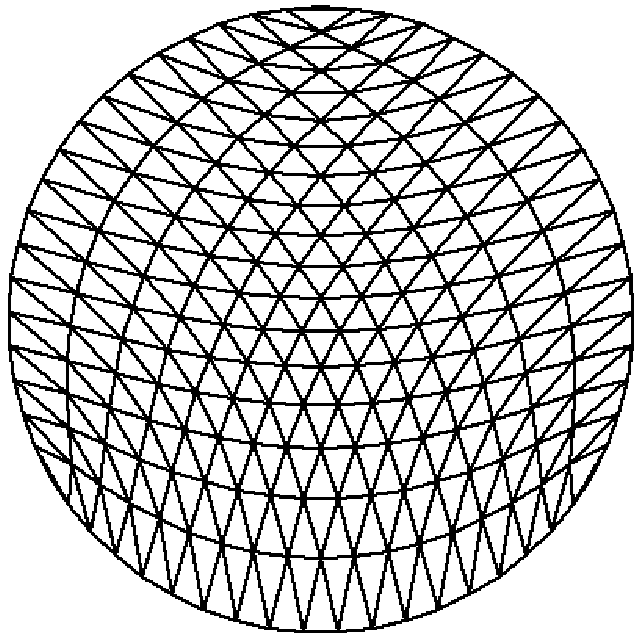
\includegraphics[width=4cm]{tmesh1}}
      \caption{Das mit der Sechs-Punkt-Interpolationstechnik berechnete Netz.}\label{tmesh1}
    \end{figure}
    Die Verallgemeinerung des Laplaceoperators ist naheliegend. Es wird dabei der
    Schwerpunkt $C$ der  sechs Nachbarknoten benutzt. Das mit dem Laplaceoperator gegl"attete Netz 
    ist in Abbildung~\ref{tmesh2} dargestellt.
    \begin{figure}[htb]
      \centerline{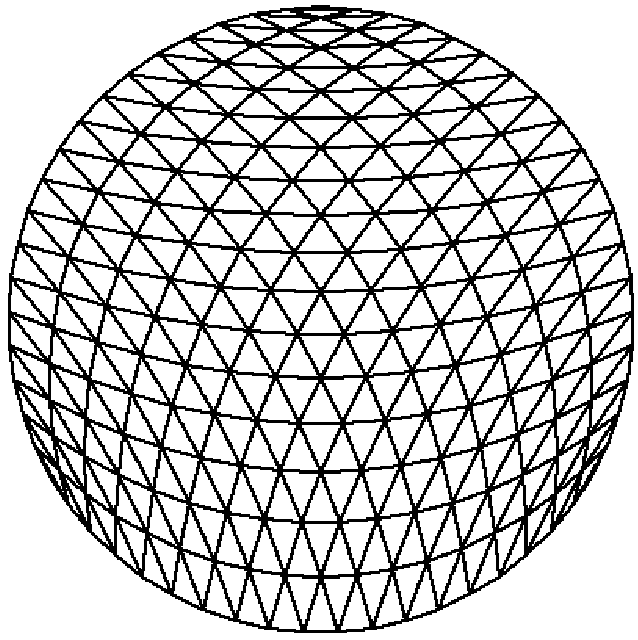
\includegraphics[width=4cm]{tmesh2}}
      \caption{Das mit dem Laplaceoperator gegl"attete Netz.}\label{tmesh2}
    \end{figure}
    F"ur die Berechnung der optimalen Position eines inneren Knoten ist der
    Acht-Punkt-Algorithmus nicht geeignet, da er nicht an die
    Dreieckstopologie angepa"st ist. Deswegen wird ein Neun-Punkt-Algorithmus
    verwendet. Betrachten wir einen inneren Knoten $P_0$, der von neun 
    Nachbarknoten $P_1,\ldots,P_9$ umgeben ist (siehe Abbildung~\ref{neun}).
    \begin{figure}[htb]
      \centerline{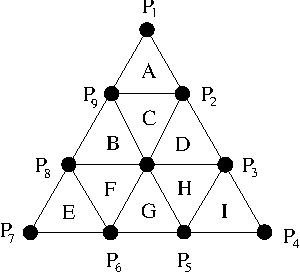
\includegraphics{neun}}
      \caption{Neun Nachbarknoten eines inneren Knotens $P_0$}\label{neun}
    \end{figure}
    Um ein Netz mit gleich gro"sen Fl"achenelementen zu erhalten, fordern wir, da"s die Fl"achen 
    folgende Gleichungen 
    \begin{eqnarray}
      A + C + D + H + I &=& A + C + B + E + F, \\
      E + F + G + H + I &=& A + C + B + E + F,
    \end{eqnarray}
    oder "aquivalent
    \begin{eqnarray}
      D + H + I &=& B + E + F, \\
      G + H + I &=& A + C + B
    \end{eqnarray}
    erf"ullen. Wenn man die beiden Gleichungen in den Koordinaten der Nachbarknoten und der idealen
    Position $C$ ausdr"uckt, bekommt man zwei lineare Gleichungen f"ur $x_c$ und $y_c$. Die L"osungen sind
    \begin{eqnarray}
      x_c & = & \frac{e d - f b}{a d - c b} \\
      y_c & = & \frac{a f - c e}{a d - c b},
    \end{eqnarray}
    wobei
    \begin{eqnarray*}
      a &=& y_5 + y_6 - y_2 - y_9 \\
      b &=& x_2 + x_9 - x_5 - x_6 \\
      c &=& y_6 + y_8 - y_2 - y_3 \\
      d &=& x_2 + x_3 - x_6 - x_8 \\
      e &=& x_7 (y_6 - y_8) + y_7 (x_8 - x_6) + x_4 (y_5 - y_3) + y_4 (x_3 - x_5) \\ 
	    & & + x_9 y_8 - y_9 x_8 + x_2 y_3 - x_3 y_2 \\
      f &=& x_1 (y_9 - y_2) + y_1 (x_2 - x_9) + x_4 (y_5 - y_3) + y_4 (x_3 - x_5) \\
	    & & - x_6 y_5 + y_6 x_5 + x_9 y_8 - y_9 x_8
    \end{eqnarray*}
    gesetzt sind.

    Das mit diesen Bedingungen optimierte Netz ist in Abbildung~\ref{tmesh3} dargestellt.
    Die Randknoten wurden dabei nicht bewegt. 
    \begin{figure}[htb]
      \centerline{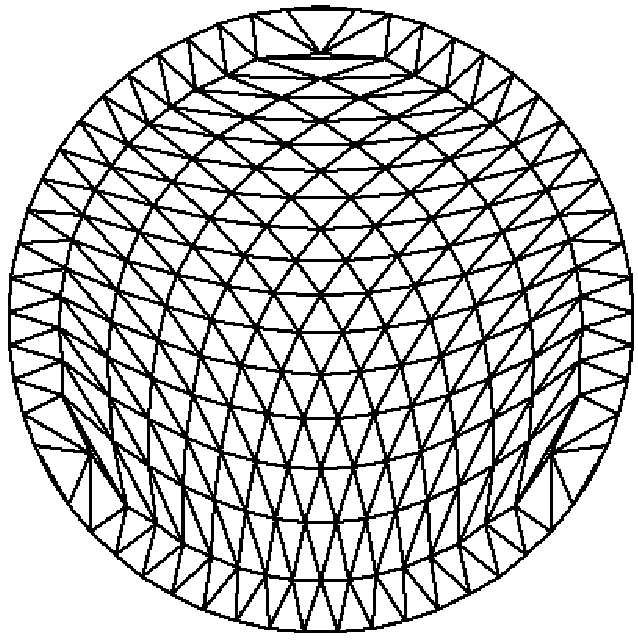
\includegraphics[width=4cm]{tmesh3}}
      \caption{Das bei der Abbildung eines Dreiecks auf einen Kreis entstandene Netz. Das Netz wurde dabei so optimiert, da"s alle Fl"achenelemente gleich gro"s sind.}\label{tmesh3}
    \end{figure}
    Betrachten wir einen Randknoten $P_0$ in Abbildung~\ref{dreirand}. 
    \begin{figure}[htb]
      \centerline{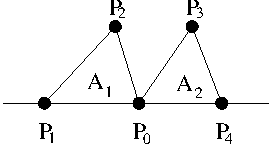
\includegraphics{dreirand}}
      \caption{Der Randknoten hat f"unf Nachbarknoten}\label{dreirand}
    \end{figure}
    Die Forderung, da"s $A=B$ gilt, liefert
    eine lineare Gleichung f"ur die Koordinaten $x_c$ und $y_c$
    \begin{equation}  a  x_c + b  y_c = e, \end{equation}
    wobei
    \begin{eqnarray*}
      a & = & y_1 - y_2 - y_3 + y_4,                                \\
      b & = & -x_1 + x_2 + x_3 - x_4,								\\
      e & = & x_3  y_4 - y_3  x_4 - ( x_1  y_2 - y_1  x_2 )
    \end{eqnarray*}
    gesetzt sind. Die ideale Position $C$ f"ur den Randknoten wird dann wie im vorherigen Beispiel berechnet.
    Das so optimierte  Netz ist in Abbildung~\ref{tmesh4} gezeigt.
    \begin{figure}[htb]
      \centerline{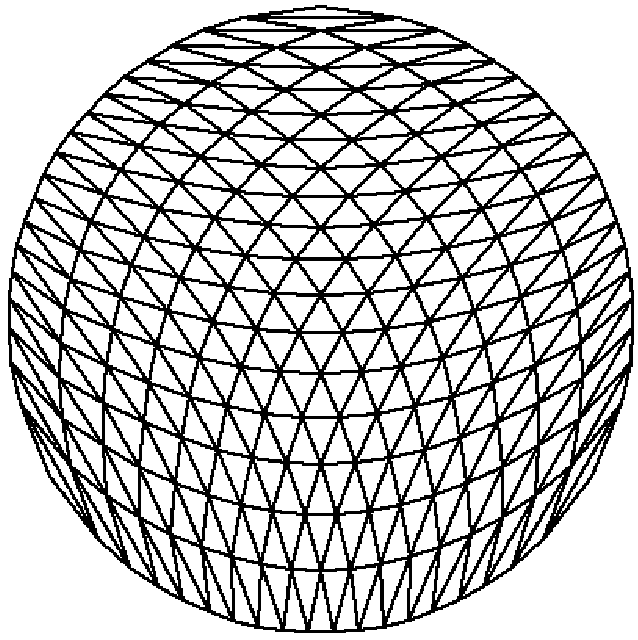
\includegraphics[width=4cm]{tmesh4}}
      \caption{Das bei der Abbildung eines Dreiecks auf einen Kreis entstandene Netz. Das Netz wurde dabei so optimiert, da"s alle Fl"achenelemente gleich gro"s sind.}\label{tmesh4}
    \end{figure}
%%
%%  Netz f"ur allgemeine Wellenfront
%%
  \subsection{Netze f"ur allgemeine Wellenfronten}
    Betrachten wir das Problem, zwei Wellenfronten $f_1$ und $f_2$ mit beliebigen Intensit"atsverteilungen 
    mit Hilfe eines diffraktiven Phasenelements ineinander zu transformieren. Die Phase von $f_1$ kann 
    oBdA als konstant angenommen werden. Bei der Wellenfront $f_2$ haben wir Phasenfreiheit, da uns nur die
    Intensit"atsverteilung interessiert. In diesem Abschnitt wird die Idee der finiten Elemente aus \cite{finite}
    erweitert, um auch bei beliebigen Intensit"atsverteilungen eingesetzt werden zu k"onnen.

    Die Ein- und Ausgabesignale liegen als quadratische Arrays $input$ bzw. $output$ vor. Die Werte
    $input(x_{pix}, y_{pix})$ und $output(x_{pix}, y_{pix})$ geben die Amplitude des 
    Eingabe- bzw. des Ausgabesignals im Punkt $(x_{pix},y_{pix})$ an. Die Koordinaten $x_{pix}$ und $y_{pix}$
    stammen aus dem Bereich $\left[0,\ldots, size-1\right]$, wobei $size$ die Gr"o"se der Arrays ist. 
    F"ur die Ein- und Ausgabesignale werden topologisch "aquivalente Netze mit demselben Algorithmus generiert. 
    
    Als Startwert nehmen wir ein quadratisches Netz mit Rechteckstopologie, das in gleich gro"se quadratische 
    Fl"achenelemente unterteilt ist. Die Koordinaten dieses Netzes stammen aus dem Bereich 
    $\left[0,1\right]$. In einem iterativen Proze"s werden die Knoten solange bewegt, bis jedes 
    Fl"achenelement die gleiche Energie enth"alt.

    Um die Energie in einem Fl"achenelement zu messen, m"ussen wir die Koordinaten seiner Knoten 
    $(x_k,y_k)$ mit $x_k,y_k \in \left[0, 1\right]$ in Pixelkoordinaten $(x^{k}_{pix},y^{k}_{pix})$ mit 
    $x^k_{pix}, y^k_{pix} \in \left[0,\ldots,size-1\right]$ entsprechend der Formeln
    \begin{eqnarray}
      x^{k}_{pix} = \lfloor x_k \cdot (size-1) + 0.5 \rfloor\\
      y^{k}_{pix} = \lfloor y_k \cdot (size-1) + 0.5 \rfloor
    \end{eqnarray}  
    umrechnen. Wir bestimmen anschlie"send die Minimal- und Maximalwerte $x^{min}_{pix}, x^{max}_{pix}, y^{min}_{pix}$ 
    und $ y^{max}_{pix}$ der $x$- und $y$-Koordinaten von $(x_k,y_k)$. Wir m"ussen dann nur die
    Koordinaten $(x_{pix},y_{pix})$ mit $x_{pix}\in [ x^{min}_{pix},\ldots,x^{max}_{pix} ]$
    und $y_{pix}\in [ y^{min}_{pix},\ldots,y^{max}_{pix} ]$ ber"ucksichtigen. Wir rechnen die Pixelkoordinaten 
    $(x_{pix},y_{pix})$ in die Knotenkoordinaten $(x,y)$ mit 
    \begin{eqnarray}
      x & = & \frac{x_{pix}}{size-1} \\
      y & = & \frac{y_{pix}}{size-1}
    \end{eqnarray} 
    um und "uberpr"ufen, ob sich $(x,y)$ innerhalb des finiten Fl"achenelements befindet. 
    Falls ja, dann wird die Energie des Pixels $(x_{pix},y_{pix})$ zu der Energie des Fl"achenelements dazuaddiert.

    Um festzustellen, ob sich ein Punkt $Q=(Q.x, Q.y)$ innerhalb eines Polygons $P$ befindet wird das 
    Halbstrahlverfahren aus \cite{schmidt}
    verwendet. Der Algorithmus macht sich einen Satz zunutze, der besagt, da"s jede Halbgerade, beginnend mit $Q$, 
    das Polygon $P$ genau dann mit ungerader Anzahl von Schnittpunkten schneidet, wenn $Q$ im Inneren von $P$ liegt. 
    Der Algorithmus testet alle Kanten
    auf Schnitt mit der bei $Q$ beginnenden Halbgeraden und "uberpr"uft die Schnittzahl gem"a"s dem obigen Satz.

    Um numerische Probleme beim Schnittpunkttest zu vermeiden werden Schnittpunkte ausschlie"slich dann gez"ahlt, wenn
    die betrachtete Strecke einen echten Schnittpunkt mit dem Halbstrahl hat. Zus"atzlich sind nur noch die
    Gebietswechsel zu betrachten. Hierf"ur werden folgende Pr"adikate definiert, von denen auch der folgende
    Algorithmus Gebrauch macht:
    \begin{enumerate}
      \item $P_i P_{i+1}$ schneidet den Halbstrahl genau dann, wenn gilt:
        $$ ((P_i.y > Q.y) \wedge (P_{i+1}.y < Q.y)) \vee ((P_i.y < Q.y) \wedge (P_{i+1} > Q.y)) $$
        und f"ur den Schnittpunkt $(x_0, Q.y)$ gilt: $x_0 > Q.x$.
      \item $P_i P_{i+1}$ erzeugt einen Gebietswechsel genau dann, wenn:
        \begin{eqnarray*}
          ((P_i.y = Q.y) \wedge (P_i.x > Q.x) \wedge (P_{i+1} < Q.y)) & \vee & \\
          ((P_{i+1}.y = Q.y) \wedge (P_{i+1}.x > Q.x) \wedge (P_i < Q.y)). & &
        \end{eqnarray*}
    \end{enumerate}
    Gebietswechsel liegen also nur bei solchen Kanten vor, deren einer Eckpunkt rechts von $Q.x$ auf dem Halbstrahl und deren
    anderer Endpunkt unter dem Halbstrahl liegt. Der Algorithmus lautet:
    \begin{verbatim}
 begin
   zaehler := 0;
   for alle Kanten k = P_i P_i+1 do begin
     if (k schneidet Halbstrahl) or (k erzeugt Gebietswechsel) 
       then zaehler++;
   end;
   in := ((zaehler mod 2) = 1);
 end;
    \end{verbatim}
    Betrachten wir einen inneren Knoten $P_0$ (siehe Abbildung~\ref{acht}), der von den acht Nachbarn 
    $P_1,\ldots,P_8$ umgeben ist. Wir bestimmen die ideale Position $C(x_c,y_c)$ f"ur den inneren Knoten $P_0$, so da"s 
    die Energie der vier Fl"achenelemente gleich gro"s ist. Dazu gewichten wir die Fl"achen $A_1,\ldots,A_4$ mit der
    in ihnen jeweils enthaltenen Energien $a,\ldots,d$. Die Bedingungen lauten dann
    \begin{eqnarray}
      a A_1 + b A_2 & = & c A_3 + d A_4, \\
      a A_1 + c A_3 & = & b A_2 + d A_4.
    \end{eqnarray}
    Wenn wir diese Bedingungen mit den Koordinaten der acht Nachbarknoten $P_1,\ldots,P_8$ und
    der idealen Position $C(x_x, y_c)$ ausdr"ucken, erhalten wir zwei lineare Gleichungen f"ur die
    Unbekannten $x_c$ und $y_c$. Dieses Gleichungssystem wurde mit Mathematica gel"ost. Die L"osungen
    wurden noch mit Magma vereinfacht. Die neue Position $P_0'$ berechnet sich wie in der Gleichung~\ref{verschiebung}.

    Die Randknoten m"ussen auch wie in den vorigen Beispielen getrennt behandelt werden. 
    Betrachten wir einen Randknoten $P_0$, der kein Eckpunkt ist (siehe Abbildung~\ref{rechtran}). 
    Die Bedingung, da"s die beiden Fl"achenelemente die gleiche Energie enthalten, lautet
    \begin{eqnarray}
      a A_1 = b A_2.
    \end{eqnarray}
    Mit dieser Bedingung ist eine Gerade festgelegt, auf der sich die ideale Posi\-tion $C$ befindet. Eine zweite 
    Bedingung, die die Position $C$ eindeutig festlegt, ergibt sich aus der Tatsache, da"s sie auf dem Rand liegen mu"s.
    Da wir ein quadratisches Signalfenster benutzen, sind die R"ander achsenparallele Strecken.

    Betrachten wir zwei Beispiel f"ur Netze, die mit der oben beschriebenen Methode berechnet wurden. In der
    Abbildung~\ref{marmesh} ist das zur Marilyn geh"orende Netz gezeigt. Man kann deutlich erkennen, da"s die Maschen
    die "uber dem Mund liegen gr"o"ser sind als die anderen, weil die Energie dort sehr klein ist. 
    \begin{figure}[htb]
      \centerline{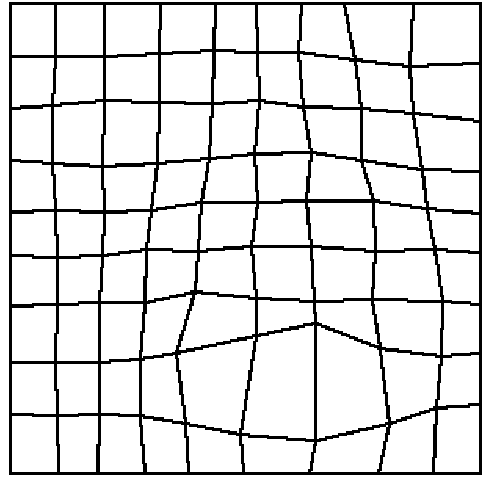
\includegraphics[width=4cm]{MarMesh}}
      \caption{Das zu Marilyn geh"orende Netz.}\label{marmesh}
    \end{figure}
    In der Abbildung~\ref{gaumesh} ist das zu einem zweidimensionalen Gauss-Signal geh"orende Netz zu sehen. Die
    Maschengr"o"se nimmt zur Mitte hin ab, da die Energie in der Mitte sehr gro"s ist und nach au"sen
    exponentiell abnimmt.
    \begin{figure}[htb]
      \centerline{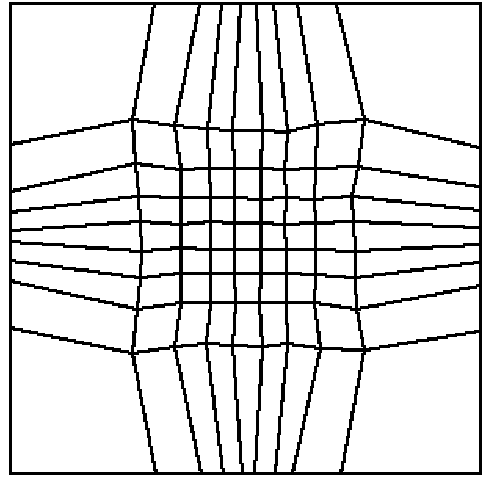
\includegraphics[width=4cm]{GauMesh}}
      \caption{Das zu einem zweidimensionalen Gauss-Signal geh"orende Netz.}\label{gaumesh}
    \end{figure}
    Es soll ein Netz f"ur das Signal in Abbildung~\ref{insep} mit $s=10$ generiert werden.
    \begin{figure}[htb]
      \centerline{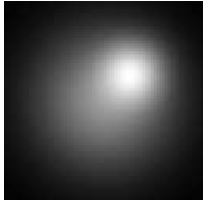
\includegraphics[width=4cm]{insep}}
      \caption{Ein inseparables Signal.}\label{insep}
    \end{figure}
    In der Abbildung~\ref{konvergenz} ist die Standard- und maximale Abweichung der in den 
    Netzmaschen enthaltenen Energien von der optimalen Energie in Abh"angigkeit der Anzahl der
    Iterationen aufgetragen.
     \begin{figure}[htb]
      \centerline{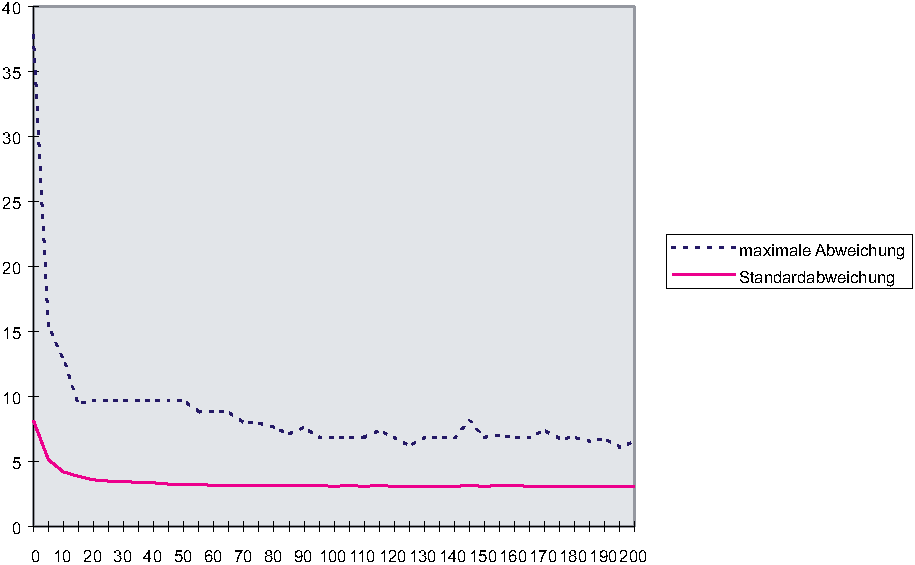
\includegraphics[width=8cm]{konvergenz}}
      \caption{Konvergenzverhalten in Abh"angigkeit der Iterationen.}\label{konvergenz}
    \end{figure}

  \subsection{Bestimmung der Phasenfunktion}  
    In diesem Abschnitt zeigen wir, wie die Phasenfunktion $\phi(x,y)$ des Phasenelements mit 
    den zuvor generierten Netzen berechnet werden kann. Es wird die Idee aus \cite{phase} verwendet.
    F"ur jedes $(i,j)$-Paar haben wir die Koordinaten
    $(x^{ij},y^{ij})$ des zugeh"origen Knotens in der Eingabeebene $in(i,j)$ und die Koordinaten 
    $(\phi_x^{ij},\phi_y^{ij})$ des zugeh"origen Knoten $out(i,j)$ in der Ausgabe\-ebene. Wir m"ussen 
    ein Phasenelement realisieren, da"s die Energie der finiten Fl"achenelemente in der Eingabeebene $E$ 
    in die jeweils korrespondierenden finiten Fl"achenelemente in der Ausgabeebene $A$ ablenkt.

    Wir nehmen an, da"s die Phasenfunktion $\phi(x,y)$ des Phasenelements durch ein bivariates Polynom vom 
    Grad $D-1$ angen"ahrt werden kann, d.h.
    $$ \phi(x,y) = \sum_{k=0}^{D-1}\sum_{l=0}^{D-1-k} a_{kl}\cdot x^k y^k, $$
    wobei die $a_{kl}$ die Koeffizienten des Polynoms in Abh"angigkeit von Koordinaten der
    $in$- und $out$-Knoten zu bestimmen sind. Der Koeffizient $a_{00}$ kann oBdA $a_{00}=0$ gesetzt werden,
    da die konstante Phase uninteressant ist. Nach der Methode der station"aren Phase mu"s f"ur 
    die Phasenfunktion $\phi(x,y)$ eines Phasenelements
    $$ \nabla \phi(x,y) = c \cdot T(x,y)$$
    gelten, damit das Phasenelement die geometrische Transformation $T$ realisiert. 
    F"ur die Phasenfunktion $\phi(x,y)$ mu"s also 
    \begin{eqnarray*}
      \partial\phi(x_{ij},y_{ij})/\partial x & = & c\cdot \phi_x^{ij}, \\
      \partial\phi(x_{ij},y_{ij})/\partial y & = & c\cdot \phi_y^{ij} 
    \end{eqnarray*}
    f"ur alle $(i,j)$-Paare gelten. Die partiellen Ableitungen des Polynoms $\phi(x,y)$ sind
    \begin{eqnarray*}
      {\partial\phi\over\partial x} & = & 
      \sum_{k=0}^{D-1}\sum_{l=0}^{D-1-k} k\cdot a_{kl}\cdot x^{k-1} y^l, \\
      {\partial\phi\over\partial y} & = &
      \sum_{k=0}^{D-1}\sum_{l=0}^{D-1-k} l\cdot a_{kl}\cdot x^k y^{l-1}.
    \end{eqnarray*}
    Wir bestimmen den Koeffizientenvektor $\underbar{a}=(a_{kl})$ mit der
    Methode der kleinsten Quadrate angewandt auf die partiellen Ableitungen
    $\partial\phi/\partial x$ und $\partial\phi/\partial y$, deren Werte
    f"ur alle $(i,j)$-Paare bekannt sind. Dazu definieren wir eine Funktion $g(\underbar{a})$ durch
    $$ g(\underbar{a}) = \sum_{i,j}\left\{\left[\left(
                           \sum_{k,l} k\cdot a_{kl}\cdot x_{ij}^{k-1}y_{ij}^l\right)
                           - \phi_x^{ij}\right]^2 + 
                                   \left[\left(
                           \sum_{k,l} l\cdot a_{kl}\cdot x_{ij}^k y_{ij}^{l-1}\right)
                           - \phi_y^{ij}\right]^2
                         \right\}.
    $$
    Um $g(\underbar{a})$ zu minimieren, m"ussen die partiellen Ableitungen
    \begin{eqnarray*}
    {\partial g\over \partial a_{kl}} =
       \sum_{ij} &2&\left[\left(
                          \sum_{m,n} m\cdot a_{mn}\cdot x_{ij}^{m-1}y^n\right) -
                              \phi_x^{ij}\right]\cdot k\cdot x_{ij}^{k-1} y_{ij}^l + \\
                 &2&\left[\left(
                          \sum_{m,n} n\cdot a_{mn}\cdot x_{ij}^m y^{n-1}\right) -
                              \phi_y^{ij}\right]\cdot l\cdot x_{ij}^k y_{ij}^{l-1}
    \end{eqnarray*}
    f"ur alle $a_{kl}$ verschwinden, d.h.
    $$ {\partial g(\underbar{a}) \over\ \partial a_{kl}} \stackrel{!}{=} 0. $$
    Das ist "aquivalent zu 
    $$ \sum_{i,j}\left( k\cdot x_{ij}^{k-1}y_{ij}^l\cdot \phi_x^{ij} +
                        l\cdot x_{ij}^ky_{ij}^{l-1}\cdot \phi_y^{ij} \right) = $$
    $$ \sum_{i,j}\sum_{m,n}\left( m\cdot a_{mn}\cdot x_{ij}^{m-1} y_{ij}^n \cdot k \cdot x_{ij}^{k-1} y_{ij}^l +
                                  n\cdot a_{mn}\cdot x_{ij}^m y_{ij}^{n-1} \cdot l \cdot x_{ij}^k y_{ij}^{l-1}
                           \right). $$
    Das ist ein lineares Gleichungssystem f"ur die Unbekannten $a_{mn}$. Die 
    Eintr"age $m_{row,col}$ der zugeh"origen Matrix sind 
    \begin{equation}
     m_{row, col} = \sum_{i,j=0}^{s-1} m \cdot k \cdot x_{ij}^{m-1+k-1} \cdot y_{ij}^{n+1} +
                                       n \cdot l \cdot x_{ij}^{m+k} \cdot y_{ij}^{n-1+l-1},
    \end{equation}
    wobei
    \begin{eqnarray*}
       row & = & l \cdot (2 D-l+1)/2+k,\\
       col & = & n \cdot (2 D-n+1)/2+m
    \end{eqnarray*}
    gesetzt sind. Die Eintr"age $m_{row, D(D+1)/2}$ des zugeh"origen L"osungsvektors sind
    \begin{equation}
      m_{row, D(D+1)/2} = \sum_{i,j=0}^{s-1} k \cdot \phi_x^{ij} \cdot x_{ij}^{k-1} \cdot y_{ij}^l +
                                             l \cdot \phi_y^{ij} \cdot x_{ij}^k     \cdot y_{ij}^{l-1}.
    \end{equation}
    Wir l"osen das Gleichungssystem mit der Gausselimination und erhalten die L"osungen der
    Koeffizienten $a_{mn}$. Damit ist die Phasenfunktion $\phi(x,y)$ bekannt und wir k"onnen das 
    Phasenelement angeben.
    
\section{Vergleich }
  Um die Methode der finiten Elemente mit anderen Methoden zu vergleichen, brauchen wir geeignete 
  G"utema"se, mit denen sich die Qualit"at diffraktiver Phasenelemente quantitativ beschreiben l"a"st. 
  Das Signal-Rausch-Verh"altnis beschreibt, wie der Name schon sagt, das Verh"altnis
  der Energie des Signals zur Energie des Rauschens, welches das Signal "uberlagert. Das Signal
  ist in diesem Fall das gew"unschte Ausgabesignal $f_2$, das durch die Funktion 
  $f_2 : \R^2 \rightarrow \C$ gegeben ist. Das Rauschen ergibt sich aus der Abweichung
  des mit diffraktiven Phasenelement (DPE) erzeugten Signals 
  $f(x)=\mathcal{F}\left\{f_1 T_{DPE}\right\}(x)$ vom 
  gew"unschten Ausgabesignal $f_2$, wobei lediglich die Energie innerhalb eines begrenzten Bereichs, 
  dem Signalfenster $W_{Signal}$, betrachtet wird.

  Die SNR wird f"ur das gew"unschte Ausgabesignal $f_2$ und das Signal $f$, die beide 
  als Intensit"atssignale betrachtet werden, wie folgt definiert:
  $$ \snr{f_2}{f} = \frac{\norm{f}^2} {\norm{\betrag{f_2}-\alpha\betrag{f}}^2} $$
  mit dem Skalierungsfaktor
  $$ \alpha = \frac{\skalar{\betrag{f}}{\betrag{f_2}}}{\norm{f}^2}. $$
  Dieser Skalierungsfaktor wird ben"otigt, da die Skalierung unwichtig f"ur den 
  Informationsgehalt des Signals ist, den die SNR messen soll. Die SNR ist
  ein Ma"s f"ur die "Ubereinstimmung des vom diffraktiven Element erzeugten Signals $f$
  und des gew"unschten Signals $f_2$.

  Die Beugungseffizienz $\eta$ ist durch den Quotienten der Energie der durch das
  diffraktive Phasenelement erzeugten Wellenfront $f$ innerhalb des 
  Signalfensters $W_{Signal}$ und der Energie der Beleuchtungswelle 
  $f_1$ im DE-Fenster $W_{DE}$ gegeben.
  $$ \eta = \frac{\norm{f}}{\parallel f_1 \parallel_{W_{DE}}^2} $$
  Die Beugungseffizienz ist damit der Anteil der Energie der Beleuchtungswelle, die
  das Signalfenster erreicht und damit ein Ma"s f"ur die Energieausnutzung des 
  diffraktiven Elements. 

  Es folgt eine Gegen"uberstellung der verschiedenen Methoden f"ur die Berechnung
  eines Startwerts f"ur den IFTA. Zum Vergleich berechnete der IFTA von den Startwerten ausgehend ein
  kontinuierliches Phasenelement, wobei 10 Iterationen zur Verbesserung der Beugungseffizienz
  und 20 Iterationen zur Verbesserung der SNR durchgef"uhrt wurden.

  Bei der Abbildung eines Kreises mit konstanter Intensit"at auf Marilyn liefert
  die Methode der finiten Fl"achenelemente den besten Startwert.

  \begin{center}{\large Kreis $\mapsto$ Marilyn} \\
  \begin{tabular}{|c|l|l|}\hline 
    Verfahren   & SNR in dB & $\eta$ in \% \\ \hline\hline
    SepOp	 &  19,3   & 78,6 \\
    Kugel	 &  16,9   & 75,1 \\
    Zufall       &  13,8   & 68,9 \\
    Mesh	 &  20,83  & 79	  \\ \hline 
  \end{tabular}\end{center}

  Bei der Abbildung des inseparablen Signals in der Abbildung~\ref{insep} auf Marilyn liefert
  die Methode der finiten Fl"achenelemente das beste Signal-Rausch-Verh"altnis.
   
  \begin{center}{\large insep	$\mapsto$ Marilyn} \\
  \begin{tabular}{|c|l|l|} \hline  
    Verfahren   & SNR in dB & $\eta$ in \% \\ \hline\hline
    SepOp	& 32,8	    & 92,1         \\	
    Kugel	& 31,1	    & 83	   \\    
    Zufall	& 30,6	    & 84,1	   \\
    Mesh        & 35.81	    & 86	   \\ \hline
  \end{tabular}\end{center}

  Bei der Abbildung des Quadrats mit konstanter Intensit"at auf Marilyn liefert
  die Methode der finiten Fl"achenelemente das beste Signal-Rausch-Verh"altnis.
\newpage
  \begin{center}{\large Quadrat $\mapsto$ Marilyn} \\		
  \begin{tabular}{|c|l|l|} \hline
    Verfahren   & SNR in dB & $\eta$ in \% \\ \hline\hline
    SepOp	& 20,8	& 79,1	    \\
    Kugel	& 20,4	& 77,8	    \\
    Zufall	& 13,9	& 68,2	    \\
    Mesh	& 20.52	& 78	    \\ \hline
  \end{tabular}\end{center} 

  Bei der Abbildung eines zweidimensionalen Gauss-Signals auf Marilyn liefert
  der Separabilisierungsoperator den besten Startwert.

  \begin{center}{\large Gauss $\mapsto$ Marilyn} \\	
  \begin{tabular}{|c|l|l|} \hline
    Verfahren   & SNR in dB & $\eta$ in \% \\ \hline\hline
    SepOp	& 31,4	& 92,5 \\	
    Kugel	& 27,5	& 84,2 \\	
    Zufall	& 23,6	& 84   \\	
    Mesh	& 29.89	& 83   \\ \hline
  \end{tabular}\end{center}

  Bei der Abbildung eines Kreises auf ein Quadrat ist die Methode der finiten
  Fl"achenelemente schlechter als die adaptierte Kugelphase.  

  \begin{center}{\large Kreis	$\mapsto$ Quadrat} \\
  \begin{tabular}{|c|l|l|} \hline
    Verfahren   & SNR in dB & $\eta$ in \% \\ \hline\hline
    SepOp	& 24,9	 & 82,6	 \\
    Kugel	& 25,9	 & 81,8	 \\
    Zufall	& 14,6	 & 71,4	 \\
    Mesh	& 18.26	 & 76	 \\ \hline
  \end{tabular}\end{center} 
\section{Schlu"sbetrachtung}
  Die Methode der finiten Elemente ist eine neue Methode, geeignete Startwerte
  f"ur IFTA zu berechnen. Diese Methode liefert bei einigen F"alle bessere Ergebnisse
  als die bisherigen Verfahren. Ein Nachteil der Methode der finiten Elemente im
  Vergleich zum SepOp ist, da"s die Parameter $s$, die Anzahl der Knoten, und $D$, der
  Grad des Polynoms, richtig gew"ahlt werden m"ussen. Bei den obigen Beispielen
  wurden viele Parameterkombinationen ausprobiert und jeweils das beste Ergebnis
  genommen. Das ist aufwendig im Vergleich zum Separabilisierungsoperator, bei dem keine
  Parameter festgelegt werden
  m"ussen. Allgemein l"a"st sich sagen, da"s die Ergebnisse besser werden, je mehr Knoten
  verwendet werden. Allerdings darf man nicht zu viele Knoten nehmen, da ihre Koordinaten
  in Pixel umgerechnet werden. Der Grad $D$ sollte kleiner gleich der H"alfte der
  Knotenanzahl $s$ gew"ahlt werden, weil sonst "Uberschwinger bei der
  Approximation entstehen.   


\newpage
\begin{thebibliography}{10}
  \bibitem[Aag93]{diplom}
    H.Aagedal, {\em Optische Implementierung linearer Transformationen mittels diffraktiver 
    Elemente}, Diplomarbeit am Institut f"ur Algorithmen und Kognitive Systeme, Universit"at Karlsruhe
  \bibitem[Aag97]{analytisch}
    H.Aagedal, M.Schmid, S.Egner, J.M"uller-Quade, Th.Beth, F.Wyrowski, {Analytical beam shaping 
    with application to laser diode arrays}, Vol. 14, No. 7/July, 1997, Journal of Optical Society of America A
    \bibitem[Atk94]{atkin}
    J.E.Atkin, {\em Finite Elements for Analysis and Design}, Academic, London, 1994
  \bibitem[Fie80]{ifta1}
    J.R.Fienup, {\em Iterative method applied to image reconstruction and to computer-generated
    holograms}, Vol. 19, 1980, Optical Engineering 
  \bibitem[Ger72]{ifta2}
    R. W. Gerchberg, W. O. Saxton, {\em A practical algorithm for the determination of phase image and diffraction
    plane pictures}, Optik (Stuttgart) 35, 237-264 (1972)
  \bibitem[Dre96]{phase}
    T. Dresel, M. Beyerlein, J. Schwider, {\em Design and fabrication of computer-generated beam-shaping holograms},
    Applied Optics 35, 4615-4621 (1996)
  \bibitem[Dre97]{finite} 
    T.Dresel, M.Beyerlein, J.Schwider, {\em Design of computer-generated beam-shaping holograms by iterative
    finite-element mesh adoption}, Applied Optics 35, 6865-6874, (1996)
  \bibitem[Schm96]{schmidt}
    Schmidt, Deussen, Kreeb, {\em Einf"uhrung in graphisch-geometrische Algorithmen}, Teubner, 1996
  \bibitem[Wyr88]{ifta3} 
    F.Wyrowski, O.Bryngdahl, {\em Iterative Fourier-transform  algorithm applied to computer holography},
    Vol. 5, No. 5/July, 1988, Journal of Optical Society of America A
\end{thebibliography}




\end{document} 
 
 
 
 
 
 
 
